\documentclass[17pt,a4paper,landscape]{extarticle}
\usepackage[margin=1.2cm]{geometry}
\usepackage{amsmath}
\usepackage{amssymb}
\usepackage{multicol}
\usepackage{enumitem}
\usepackage{tikz}
\usepackage{xcolor}
\usepackage[sfdefault,lf]{FiraSans}
\usepackage{sansmath}
\renewcommand{\familydefault}{\sfdefault}
\setlength{\parindent}{0pt}
\pagestyle{empty}
\setlength{\columnsep}{1.4cm}
\setlength{\columnseprule}{0pt}
\renewcommand{\arraystretch}{1.15}
\everymath{\displaystyle}

\begin{document}
\sffamily
\sansmath

\sansmath

\sansmath

\sansmath

{\LARGE \textbf{L02 Equivalent fractions}}\\[0.35em]
Find or identify fractions that are equivalent.

\vspace{2.6em}
{\LARGE \textbf{Foundation}}
\begin{multicols}{3}
\begin{enumerate}[
  itemsep=7.4em,
  label=\textbf{\arabic*.}, 
  labelwidth=2.2em,
  labelsep=0.75em,
  leftmargin=!,
  align=left
]
\item Write a fraction equivalent to \textbf{1/2}.
\item Write a fraction equivalent to \textbf{2/3}.
\item Write a fraction equivalent to \textbf{3/4}.
\item Write a fraction equivalent to \textbf{4/5}.
\item Are \textbf{1/2} and \textbf{2/4} equivalent?
\item Are \textbf{3/5} and \textbf{6/10} equivalent?
\item Fill in the blank: \textbf{1/3 = }\rule{1.4cm}{0.15mm}\textbf{/6}
\item Fill in the blank: \textbf{2/5 = }\rule{1.4cm}{0.15mm}\textbf{/10}
\item Fill in the blank: \textbf{3/4 = }\rule{1.4cm}{0.15mm}\textbf{/8}
\item Fill in the blank: \textbf{4/7 = 8/}\rule{1.4cm}{0.15mm}
\item {
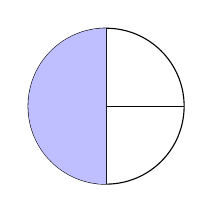
\begin{tikzpicture}[scale=0.9]
\draw (0,0) circle (1.1);
\draw (0,0)--(90:1.1);
\draw (0,0)--(180:1.1);
\draw (0,0)--(270:1.1);
\draw (0,0)--(0:1.1);
\fill[blue!25] (0,0)--(90:1.1) arc (90:180:1.1)--cycle;
\fill[blue!25] (0,0)--(180:1.1) arc (180:270:1.1)--cycle;
\end{tikzpicture}
}
\item {
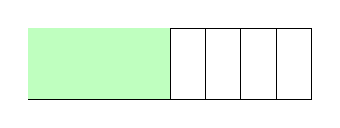
\begin{tikzpicture}[scale=0.9]
\draw (0,0) rectangle (4,1);
\foreach \x in {1,2,3} \draw (\x,0)--(\x,1);
\foreach \x in {0,0.5,...,4} \draw (\x,0)--(\x,1);
\fill[green!25] (0,0) rectangle (2,1);
\end{tikzpicture}
}
\end{enumerate}
\end{multicols}

\end{document}
